\section{Experimentos}
\label{sec:constvalidacao}
Diante dos pares de atributos selecionados na etapa (seção \ref{sec:selecaodados}), utilizou-se o método \textit{stratified-10-fold-cross-validation} (repetido dez vezes) juntamente com o \textit{ensemble DECORATE} a fim de se construir e verificar se é possível generalizar pelo menos um modelo.

Em cada verificação construi-se um modelo com diferentes frações do dataset, variando de 16 instâncias a 59 instâncias. Os resultados das avaliações podem ser vistos na Figura \ref{fig:accuracy_precision_recall} e será discutido logo a seguir na seção \ref{subsec:discumodelos}.

\section{Resultados e discussão}
\subsection{Modelos}
\label{subsec:discumodelos}
A Figura \ref{fig:accuracy_precision_recall} demonstra os resultados obtidos
através dos experimentos realizados (seção \ref{sec:constvalidacao}). Nesta, percebe-se um domínio quase absoluto da curva pontuada de aprendizado verde (médiaAltura, somaLargura - ``ma x sl''). Por esso motivo essa será a curva analisada para escolher um modelo o mais adequado possível para implantar no FIM.

\begin{figure}[!h] \centering 
  \centering
  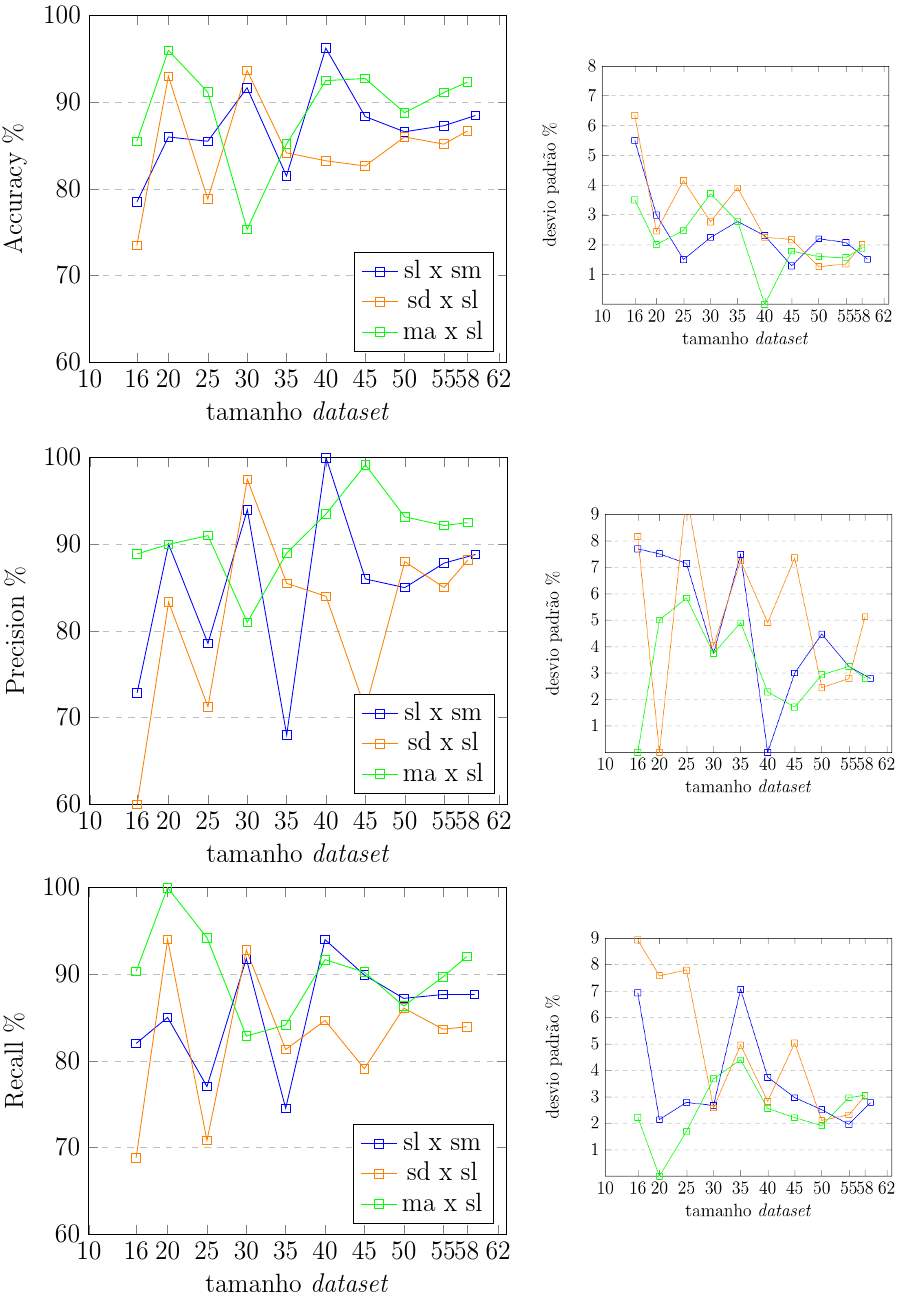
\includegraphics[width=0.8\columnwidth]{experimento/accuracy_precision_recall} 
  \caption{\textit{Accuracy}, \texit{Precision} e \textit{Recall} obtidas utilizando stratified-10-fold-crossvalidation (repetido 10 vezes) e DECORATE sobre diferentes frações do \textit{dataset} com os pares de parâmetros  selecionados na seção \ref{sec:selecaodados}.} 
  \label{fig:accuracy_precision_recall}
\end{figure}

Como o principal motivo da implantação do classificador no FIM é detectar efeitos colaterais indesejáveis, então pretende-se que o modelo tenha um alto índice de \textit{recall}, pois não se deseja que se tenha muitos falso negativos, ou seja, muitos casos classificados como não sendo efeito colateral, mas que na verdade era. Visualizando a curva percebe-se que esta têm um crescimento acentuado e depois torna-se estável a partir do dataset com 30 instâncias. Logo será realizada uma análise a partir deste ponto. Os maiores valores de \textit{recall} partindo deste ponto são aqueles quando o \textit{dataset} tem 40 ou mais instâncias, para todos estes pontos considera que se obteve um bom grau de generalização. Estes valores podem ser visualizados na Tabela \ref{table:valorescurva}. 

\begin{table}[!htp]
  \centering
  \begin{tabular}{ |l|c c c c c|}
    \hline
       {\bf \textbf{$n^o i$}} & {\bf 40} & {\bf 45} & {\bf 50} & {\bf 55} & {\bf 58} \\
    \hline
       \textbf{A, DP} & 92.5, 0 & 92.75, 1.78 & 88.8, 1.6 & 91.13, 1.56 & 92.33, 1.89 \\
    \hline
       \textbf{P, DP} & 93.5, 2.29 & 99.17, 1.71 & 93.17, 2.93 &  92.17, 3.25 & 92.5, 2.81 \\
    \hline
       \textbf{R, DP} & 91.69, 2.56 & 90.25, 2.21 & 86.33, 1.91 & 89.71, 2.97 & 92.05, 3.06 \\
    \hline
  \end{tabular}
  \caption{Valores das curvas ``ma x sl'' da Figura \ref{fig:accuracy_precision_recall} a partir do \textit{dataset} com 40 instâncias. A (\textit{Accuracy}), P (\textit{Precision}, R (\textit{Recall}), DP (Desvio Padrão), i (instâncias). Os valores A, P, R e DV estão em \%.}
  \label{table:valorescurva}
\end{table}

Finalizando a análise decidiu-se que o melhor ponto para poder se construir um classificador é o com $n^o i = 45$, pois além de se ter um alto grau de \textit{recall} e \textit{accuracy} têm-se também \textit{precision} quase de 100\%. Então, para se construir um classificador final com base neste modelo escolheu-se randomicamente 45 instâncias do \textit{dataset} de 59 instâncias e aplicou-se \textit{stratified-10-fold-cross-validation} (repetido dez vezes). Este procedimento foi repetido diversas vezes (Figura \ref{fig:apr45_dev}) até que se obtivesse um modelo que satisfizesse a expressão \ref{eq:esxpvalclass}.

\begin{equation}
  (\textit{accuracy} \geq (92.75-1.78)) \wedge (\textit{precision} \geq (99.17-1.71)) \wedge (\textit{recall} \geq 90.25)
  \label{eq:esxpvalclass}
\end{equation}

\begin{figure}[!htb] \centering 
  \centering
  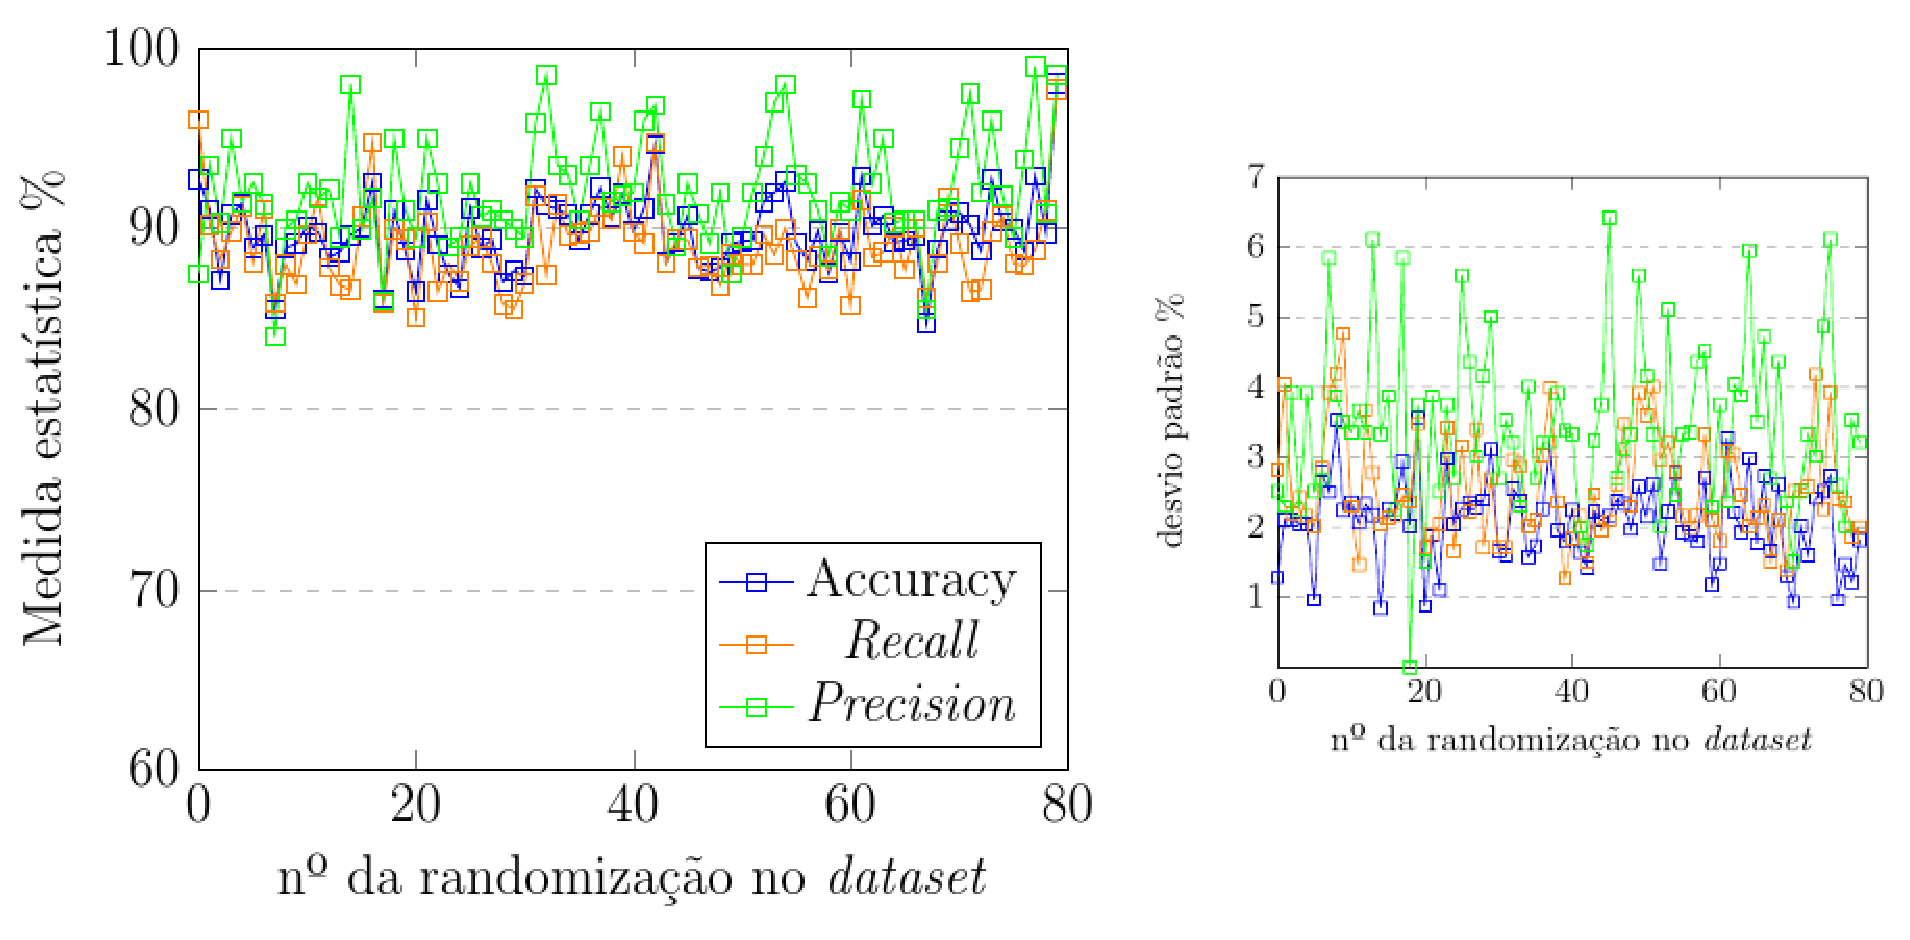
\includegraphics[width=1.0\columnwidth]{experimento/apr45_dev} 
  \caption{\textit{stratified-10-fold-cross-validation} (repetido dez vezes). 45 instâncias foram escolhidas randomicamente em cima do \textit{dataset} de 59 instâncias. Procedimento repetido até que satisfizesse a expressão \ref{eq:esxpvalclass} } 
  \label{fig:apr45_dev}
\end{figure}

O modelo que satisfez essa expressão obteve resultados que podem ser vistos na Tabela \ref{table:valmodelfinal} e este será o modelo final de classificador que será implantado no FIM. 

\begin{table}[!htp]
  \centering
  \begin{tabular}{ |l|c|c|}
    \hline
       {\bf } & {\bf } & {\bf DP \%} \\
    \hline
       \textbf{Accuracy} \% & 98.05 & 1.81 \\
    \hline
       \textbf{Precision} \% & 98.5 & 3.2 \\
    \hline
       \textbf{\textit{Recall} \%} & 97.67 & 2 \\
    \hline
  \end{tabular}
  \caption{Valores da validação do modelo final. DP (Desvio Padrão).}
  \label{table:valmodelfinal}
\end{table}

\subsection{Implantação}
O modelo final construído foi implantado no sistema de acordo com a proposta da seção \ref{sec:implmetprop}. Na Figura \ref{fig:deteccao_efeito} se tem a visão real do fluxo de execução em relação ao usuário do HNS quanto a funcionalidade ``Levar compras''. A imagem ``a)'' representa a execução quando não há efeitos colaterais indesejáveis. Enquanto que a imagem ``b)'' representa a execução quando se tem efeito colateral indesejável. 

\begin{figure}[!htb] \centering 
  \centering
  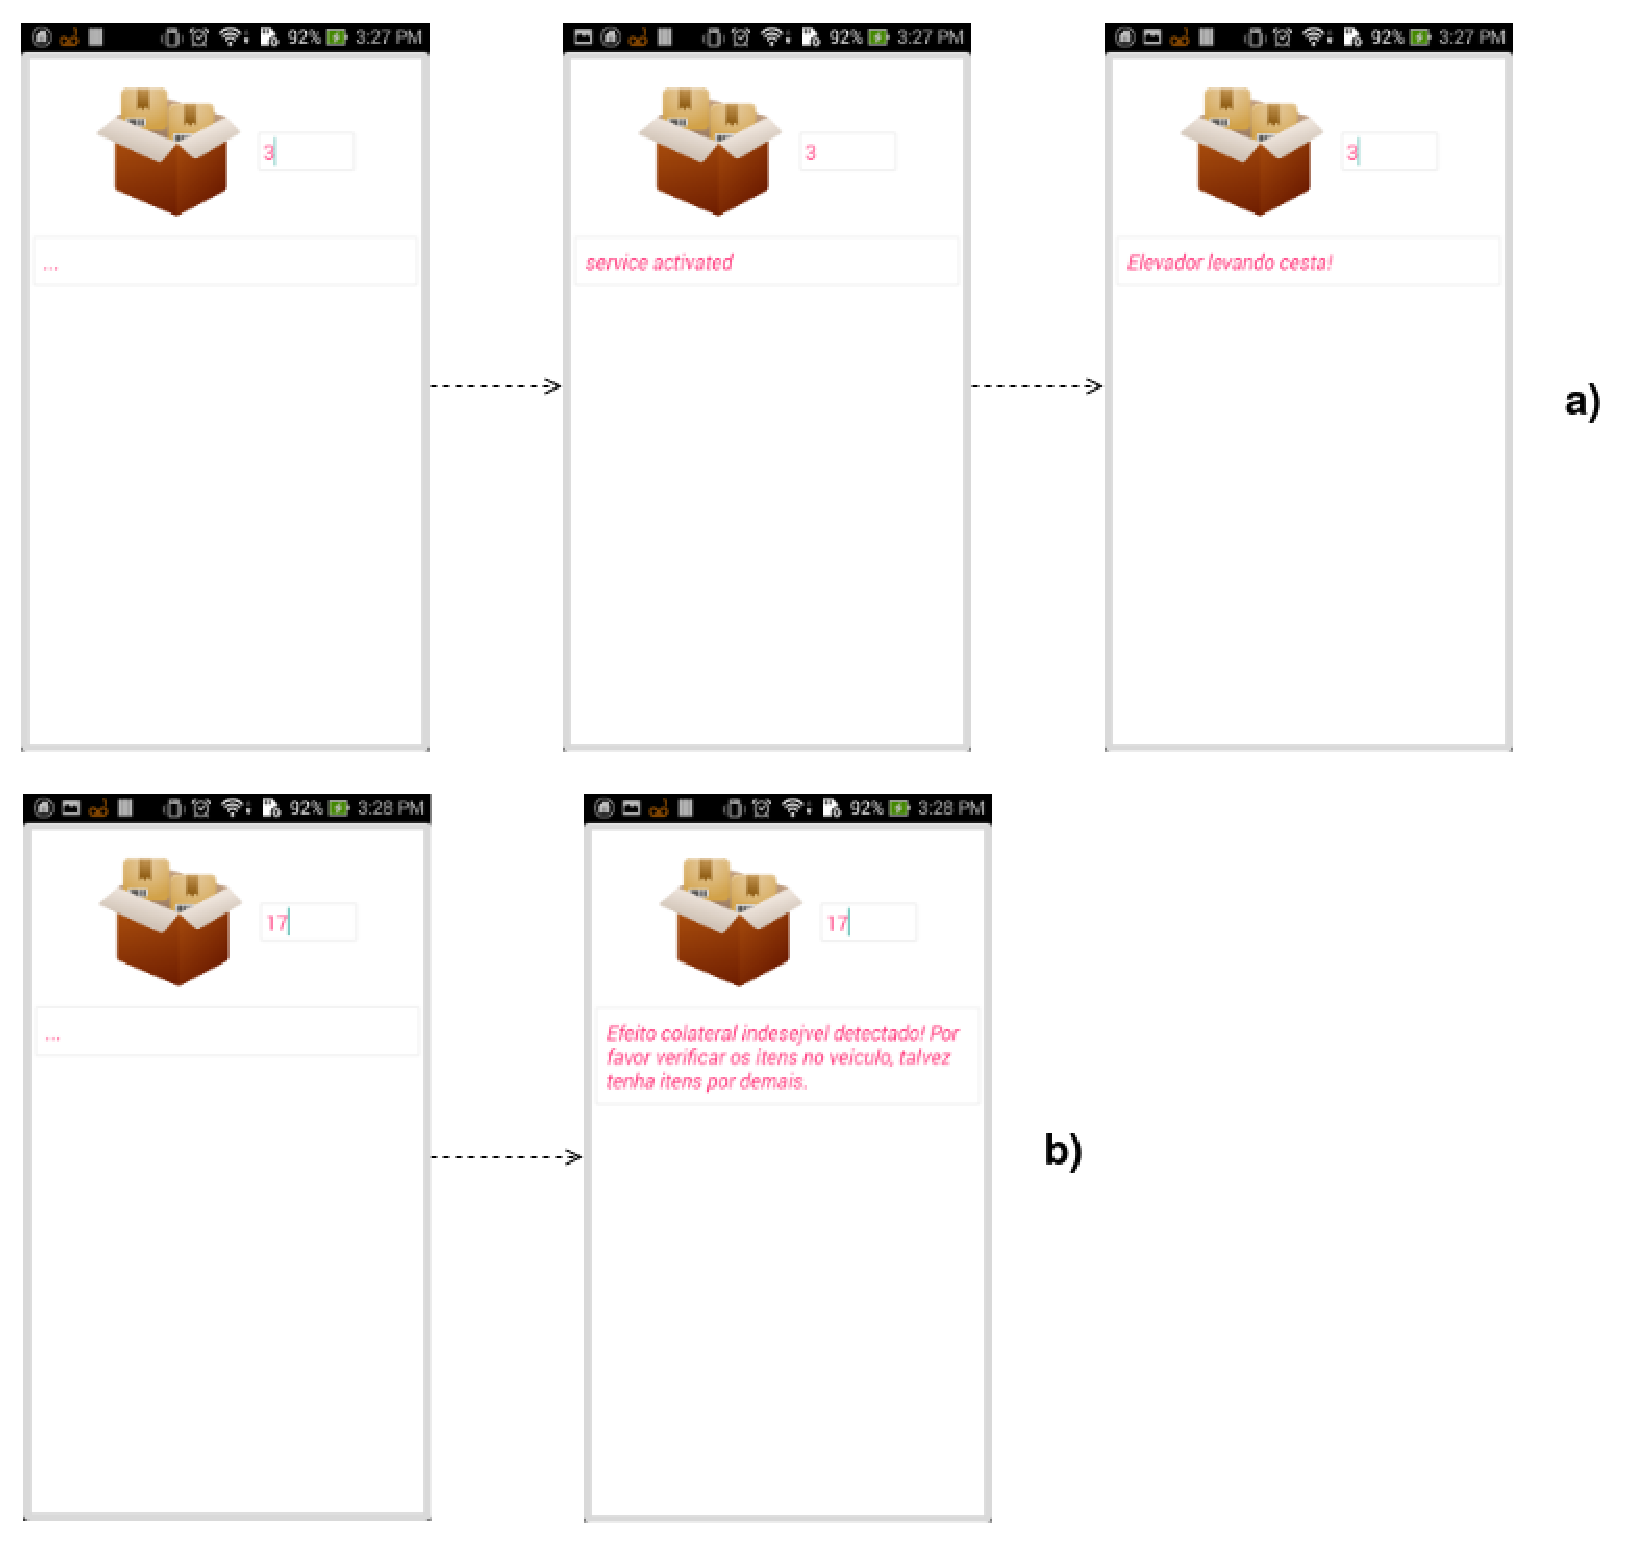
\includegraphics[width=1.0\columnwidth]{experimento/deteccao_efeito} 
  \caption{Modelo classificatório atuando no cenário ``Levar compras'' do FIM. a) Fluxo da aplicação sem efeito colateral indesejável. b) Fluxo da aplicação com efeito colateral indesejável.} 
  \label{fig:deteccao_efeito}
\end{figure}
